\documentclass[final]{beamer}

\usepackage[scale=1.24]{beamerposter}
\usetheme{confposter}
\usefonttheme{serif}

% % \usepackage[utf8]{inputenc}

% FONTS
\usepackage[T1]{fontenc}
\usepackage{tgtermes}
\usepackage{amsmath}

% Font choice 2:
\usepackage[scaled=0.92]{PTSans}
\usepackage{amssymb}
\newcommand{\mathbold}[1]{\ensuremath{\boldsymbol{\mathbf{#1}}}}
\newcommand{\mbf}[1]{\ensuremath{\boldsymbol{\mathbf{#1}}}}

% \usepackage{lmodern}

%\usefonttheme{professionalfonts}

\usepackage{scalefnt,letltxmacro}
\LetLtxMacro{\oldtextsc}{\textsc}
\renewcommand{\textsc}[1]{\oldtextsc{\fontfamily{lmr}\scalefont{1}#1}}

% \renewcommand*\ttdefault{lmvtt}
\usepackage[ttdefault=true]{AnonymousPro}

% GEOMETRY
%\usepackage[
%  paper  = letterpaper,
%  left   = 1.65in,
%  right  = 1.65in,
%  top    = 1.0in,
%  bottom = 1.0in,
%  ]{geometry}

% # COLOR

% \usepackage[usenames,dvipsnames]{xcolor}
\definecolor{shadecolor}{gray}{0.9}

% \newcommand{\red}[1]{\textcolor{BrickRed}{#1}}
% \newcommand{\orange}[1]{\textcolor{BurntOrange}{#1}}
% \newcommand{\green}[1]{\textcolor{OliveGreen}{#1}}
% \newcommand{\blue}[1]{\textcolor{MidnightBlue}{#1}}
% \newcommand{\sky}[1]{\textcolor{SkyBlue}{#1}}
% \newcommand{\gray}[1]{\textcolor{black!60}{#1}}

% SPACING and TEXT
%\usepackage[final,expansion=alltext]{microtype}
\usepackage[english]{babel}
\usepackage[parfill]{parskip}
\usepackage{afterpage}
\usepackage{framed}
\usepackage{xspace}

% LEFTBAR
\renewenvironment{leftbar}[1][\hsize]
{%
  \def\FrameCommand
  {%
    {\color{Gray}\vrule width 3pt}%
    \hspace{10pt}%
    %\hspace{0pt}\fboxsep=\FrameSep\colorbox{black!10}%
  }%
  \MakeFramed{\hsize#1\advance\hsize-\width\FrameRestore}%
}%
{\endMakeFramed}

% EDITING
% line numbering in left margin
\usepackage{lineno}
\renewcommand\linenumberfont{\normalfont
                             \footnotesize
                             \sffamily
                             \color{SkyBlue}}
% ragged paragraphs in right margin
\usepackage{ragged2e}
% TODO should i rename sidenote marginpar?
\DeclareRobustCommand{\sidenote}[1]{\marginpar{
                                    \RaggedRight
                                    \textcolor{Plum}{\textsf{#1}}}}
% paragraph counter in right margin
\newcommand{\parnum}{\bfseries\P\arabic{parcount}}
\newcounter{parcount}
\newcommand\p{%
    \stepcounter{parcount}%
    \leavevmode\marginpar[\hfill\parnum]{\parnum}%
}
% pargraph header
\DeclareRobustCommand{\parhead}[1]{\textbf{#1}~}
% paragraph helper
\DeclareRobustCommand{\PP}{\textcolor{Plum}{\P} }

% COUNTERS
%\renewcommand{\labelenumi}{\color{black!67}{\arabic{enumi}.}}
%\renewcommand{\labelenumii}{{\color{black!67}(\alph{enumii})}}
%\renewcommand{\labelitemi}{{\color{black!67}\textbullet}}

% FIGURES
\usepackage{graphicx}
\usepackage[labelfont=bf]{caption}
%\usepackage[format=hang]{subcaption}

% TABLES
\usepackage{booktabs}

% # ALGORITHMS

\usepackage[algoruled]{algorithm2e}
\setlength{\interspacetitleruled}{8pt}
\usepackage{listings}
\usepackage{fancyvrb}
\fvset{fontsize=\small}

% HYPERREF
%\usepackage[colorlinks,linktoc=all]{hyperref}
%\usepackage[all]{hypcap}
\hypersetup{citecolor=Plum}
\hypersetup{linkcolor=MidnightBlue}
\hypersetup{urlcolor=MidnightBlue}

% CLEVEREF must come after HYPERREF
\usepackage[nameinlink]{cleveref}
\newcommand{\Crefb}[1]{(\Cref{#1})}
\newcommand{\crefb}[1]{(\cref{#1})}

% ACRONYMS
\usepackage[acronym,smallcaps,nowarn]{glossaries}
\glsdisablehyper
% \makeglossaries

% COLOR DEFINITIONS
\newcommand{\red}[1]{\textcolor{BrickRed}{#1}}
\newcommand{\orange}[1]{\textcolor{BurntOrange}{#1}}
\newcommand{\green}[1]{\textcolor{OliveGreen}{#1}}
\newcommand{\blue}[1]{\textcolor{MidnightBlue}{#1}}
\newcommand{\gray}[1]{\textcolor{black!60}{#1}}

% CODE
\usepackage{minted}  % for syntax highlighting

% REFERENCES
\usepackage[
  backend=biber,
  natbib,
  doi=false,isbn=false,url=false,
  sorting=none,
  citestyle=authoryear]{biblatex}

\DeclareRobustCommand{\mb}[1]{\ensuremath{\boldsymbol{\mathbf{#1}}}}

\newcommand{\mba}{\mathbold{a}}
\newcommand{\mbb}{\mathbold{b}}
\newcommand{\mbc}{\mathbold{c}}
\newcommand{\mbd}{\mathbold{d}}
\newcommand{\mbe}{\mathbold{e}}
%\newcommand{\mbf}{\mathbold{f}}
\newcommand{\mbg}{\mathbold{g}}
\newcommand{\mbh}{\mathbold{h}}
\newcommand{\mbi}{\mathbold{i}}
\newcommand{\mbj}{\mathbold{j}}
\newcommand{\mbk}{\mathbold{k}}
\newcommand{\mbl}{\mathbold{l}}
\newcommand{\mbm}{\mathbold{m}}
\newcommand{\mbn}{\mathbold{n}}
\newcommand{\mbo}{\mathbold{o}}
\newcommand{\mbp}{\mathbold{p}}
\newcommand{\mbq}{\mathbold{q}}
\newcommand{\mbr}{\mathbold{r}}
\newcommand{\mbs}{\mathbold{s}}
\newcommand{\mbt}{\mathbold{t}}
\newcommand{\mbu}{\mathbold{u}}
\newcommand{\mbv}{\mathbold{v}}
\newcommand{\mbw}{\mathbold{w}}
\newcommand{\mbx}{\mathbold{x}}
\newcommand{\mby}{\mathbold{y}}
\newcommand{\mbz}{\mathbold{z}}

\newcommand{\mbA}{\mathbold{A}}
\newcommand{\mbB}{\mathbold{B}}
\newcommand{\mbC}{\mathbold{C}}
\newcommand{\mbD}{\mathbold{D}}
\newcommand{\mbE}{\mathbold{E}}
\newcommand{\mbF}{\mathbold{F}}
\newcommand{\mbG}{\mathbold{G}}
\newcommand{\mbH}{\mathbold{H}}
\newcommand{\mbI}{\mathbold{I}}
\newcommand{\mbJ}{\mathbold{J}}
\newcommand{\mbK}{\mathbold{K}}
\newcommand{\mbL}{\mathbold{L}}
\newcommand{\mbM}{\mathbold{M}}
\newcommand{\mbN}{\mathbold{N}}
\newcommand{\mbO}{\mathbold{O}}
\newcommand{\mbP}{\mathbold{P}}
\newcommand{\mbQ}{\mathbold{Q}}
\newcommand{\mbR}{\mathbold{R}}
\newcommand{\mbS}{\mathbold{S}}
\newcommand{\mbT}{\mathbold{T}}
\newcommand{\mbU}{\mathbold{U}}
\newcommand{\mbV}{\mathbold{V}}
\newcommand{\mbW}{\mathbold{W}}
\newcommand{\mbX}{\mathbold{X}}
\newcommand{\mbY}{\mathbold{Y}}
\newcommand{\mbZ}{\mathbold{Z}}

\newcommand{\mbalpha}{\mathbold{\alpha}}
\newcommand{\mbbeta}{\mathbold{\beta}}
\newcommand{\mbdelta}{\mathbold{\delta}}
\newcommand{\mbepsilon}{\mathbold{\epsilon}}
\newcommand{\mbchi}{\mathbold{\chi}}
\newcommand{\mbeta}{\mathbold{\eta}}
\newcommand{\mbgamma}{\mathbold{\gamma}}
\newcommand{\mbiota}{\mathbold{\iota}}
\newcommand{\mbkappa}{\mathbold{\kappa}}
\newcommand{\mblambda}{\mathbold{\lambda}}
\newcommand{\mbmu}{\mathbold{\mu}}
\newcommand{\mbnu}{\mathbold{\nu}}
\newcommand{\mbomega}{\mathbold{\omega}}
\newcommand{\mbphi}{\mathbold{\phi}}
\newcommand{\mbpi}{\mathbold{\pi}}
\newcommand{\mbpsi}{\mathbold{\psi}}
\newcommand{\mbrho}{\mathbold{\rho}}
\newcommand{\mbsigma}{\mathbold{\sigma}}
\newcommand{\mbtau}{\mathbold{\tau}}
\newcommand{\mbtheta}{\mathbold{\theta}}
\newcommand{\mbupsilon}{\mathbold{\upsilon}}
\newcommand{\mbvarepsilon}{\mathbold{\varepsilon}}
\newcommand{\mbvarphi}{\mathbold{\varphi}}
\newcommand{\mbvartheta}{\mathbold{\vartheta}}
\newcommand{\mbvarrho}{\mathbold{\varrho}}
\newcommand{\mbxi}{\mathbold{\xi}}
\newcommand{\mbzeta}{\mathbold{\zeta}}

\newcommand{\mbDelta}{\mathbold{\Delta}}
\newcommand{\mbGamma}{\mathbold{\Gamma}}
\newcommand{\mbLambda}{\mathbold{\Lambda}}
\newcommand{\mbOmega}{\mathbold{\Omega}}
\newcommand{\mbPhi}{\mathbold{\Phi}}
\newcommand{\mbPi}{\mathbold{\Pi}}
\newcommand{\mbPsi}{\mathbold{\Psi}}
\newcommand{\mbSigma}{\mathbold{\Sigma}}
\newcommand{\mbTheta}{\mathbold{\Theta}}
\newcommand{\mbUpsilon}{\mathbold{\Upsilon}}
\newcommand{\mbXi}{\mathbold{\Xi}}

\renewcommand{\d}[1]{\ensuremath{\operatorname{d}\!{#1}}}
\newcommand{\g}{\,|\,}
\renewcommand{\gg}{\,\|\,}
\newcommand\dif{\mathop{}\!\mathrm{d}}
\newcommand{\diag}{\textrm{diag}}
\newcommand{\supp}{\textrm{supp}}
\newcommand{\Gam}{\textrm{Gam}}
\newcommand{\InvGam}{\textrm{InvGam}}
\DeclareMathOperator*{\argmax}{arg\,max}
\DeclareMathOperator*{\argmin}{arg\,min}
\DeclareRobustCommand{\KL}[2]{\ensuremath{\textrm{KL}\left(#1\;\|\;#2\right)}}
\newcommand\indep{\protect\mathpalette{\protect\independenT}{\perp}}
\def\independenT#1#2{\mathrel{\rlap{$#1#2$}\mkern2mu{#1#2}}}
\newcommand{\E}[1]{\mathbb{E}\left[ #1 \right]}

\newacronym{PPL}{ppl}{probabilistic programming language}
\newacronym{GPU}{\textnormal{\uppercase{gpu}}}{graphics processing unit}

\newacronym{VAE}{vae}{variational auto-encoder}
\newacronym{RBM}{rbm}{restricted Boltzmann machine}
\newacronym{DLGM}{dlgm}{deep latent Gaussian model}
\newacronym{GAN}{gan}{generative adversarial network}
\newacronym{RNN}{rnn}{recurrent neural network}

\newacronym{VI}{vi}{variational inference}
\newacronym{MCMC}{mcmc}{Markov chain Monte Carlo}
\newacronym{MC}{mc}{Monte Carlo}
\newacronym{HMC}{hmc}{Hamiltonian Monte Carlo}
\newacronym{MAP}{map}{maximum a posteriori}
\newacronym{IWAE}{iwae}{importance-weighted auto-encoder}
\newacronym{HVM}{hvm}{hierarchical variational model}
\newacronym{KL}{kl}{Kullback-Leibler}
\newacronym{ELBO}{elbo}{\emph{evidence lower bound}}

\setbeamercolor{block title}{fg=jblue,bg=white} % Colors of the block titles
\setbeamercolor{block body}{fg=black,bg=white} % Colors of the body of blocks
\setbeamercolor{block alerted title}{fg=white,bg=dblue!70} % Colors of the highlighted block titles
\setbeamercolor{block alerted body}{fg=black,bg=dblue!10} % Colors of the body of highlighted blocks
% Many more colors are available for use in beamerthemeconfposter.sty

%-----------------------------------------------------------
% Define the column widths and overall poster size
% To set effective sepwid, onecolwid and twocolwid values, first choose how many columns you want and how much separation you want between columns
% In this template, the separation width chosen is 0.024 of the paper width and a 4-column layout
% onecolwid should therefore be (1-(# of columns+1)*sepwid)/# of columns e.g. (1-(4+1)*0.024)/4 = 0.22
% Set twocolwid to be (2*onecolwid)+sepwid = 0.464
% Set threecolwid to be (3*onecolwid)+2*sepwid = 0.708

\newlength{\sepwid}
\newlength{\onecolwid}
\newlength{\twocolwid}
\newlength{\threecolwid}
%\setlength{\paperwidth}{48in} % A0 width: 46.8in
%\setlength{\paperheight}{36in} % A0 height: 33.1in
\setlength{\sepwid}{0.024\paperwidth} % Separation width (white space) between columns
\setlength{\onecolwid}{0.301\paperwidth} % Width of one column
\setlength{\twocolwid}{0.626\paperwidth} % Width of two columns
\setlength{\threecolwid}{0.928\paperwidth} % Width of three columns
\setlength{\topmargin}{-0.5in} % Reduce the top margin size

\addtobeamertemplate{block end}{}{\vspace*{2ex}} % White space under blocks
\addtobeamertemplate{block alerted end}{}{\vspace*{2ex}} % White space under highlighted (alert) blocks

\setlength{\belowcaptionskip}{2ex} % White space under figures
\setlength\belowdisplayshortskip{2ex} % White space under equations
%-----------------------------------------------------------

\usepackage{tikz}
\usetikzlibrary{bayesnet}

\pgfdeclarelayer{edgelayer}
\pgfdeclarelayer{nodelayer}
\pgfsetlayers{edgelayer,nodelayer,main}

\definecolor{hexcolor0xbfbfbf}{rgb}{0.749,0.749,0.749}

\tikzset{>=latex}
\tikzstyle{none}   = [inner sep=0pt]
\tikzstyle{line}   = [-,
                      thick,
                      shorten <=1pt,
                      shorten >=1pt]
\tikzstyle{arrow}  = [->,
                      thick,
                      shorten <=1pt,
                      shorten >=1pt]
\tikzstyle{ardash} = [dashed,
                      ->,
                      thick,
                      shorten <=1pt,
                      shorten >=1pt]

\tikzstyle{empty}=[
                   circle,
                   opacity=0.0,
                   text opacity=1.0,
                   inner sep=0pt
                  ]

\tikzstyle{box}=[
                 rectangle,
                 fill=White,
                 thick,
                 draw=Black,
                 inner sep=7pt
                ]

\tikzstyle{filled}=[
                    circle,
                    thick,
                    fill=hexcolor0xbfbfbf,
                    draw=Black
                   ]

\tikzstyle{hollow}=[
                    circle,
                    thick,
                    fill=White,
                    draw=Black
                   ]

\tikzstyle{param}=[
                   rectangle,
                   fill=Black,
                   draw=Black,
                   inner sep=0pt,
                   minimum width=4pt,
                   minimum height=4pt
                  ]

\tikzstyle{paramhollow}=[
                         rectangle,
                         thick,
                         fill=White,
                         draw=Black,
                         inner sep=0pt,
                         minimum
                         width=4pt,
                         minimum height=4pt
                        ]

\usepackage{pgfplots}                               % PGFPLOTS baby!
\pgfplotsset{compat=newest}
\pgfplotsset{plot coordinates/math parser=false}
% \usepgfplotslibrary{statistics}


\title{Edward: A Library for Probabilistic Modeling}
\author{Dustin Tran\textsuperscript{\textdagger},
Matt Hoffman\textsuperscript{*}\textsuperscript{\ddag},
Kevin Murphy\textsuperscript{\ddag},
Eugene Brevdo\textsuperscript{\ddag},
Rif Saurous\textsuperscript{\ddag},
David Blei\textsuperscript{\textdagger}}
\institute{
\textsuperscript{\textdagger}Columbia University,
\textsuperscript{*}Adobe Research,
\textsuperscript{\ddag}Google
}

\begin{document}

\begin{frame}[t]
\begin{columns}[t]

\begin{column}{\sepwid}\end{column} % Empty spacer column

\begin{column}{\onecolwid}

\begin{alertblock}{Summary}
\begin{itemize}
  \item
Deep neural networks are popular in large part due to their

compositional nature. How do we do this for
probabilistic modeling?
  \item We describe
Edward, a new Turing-complete \acrlong{PPL}.
\item Edward builds
two representations---random variables and
inference.
\item
For example, we show how to design rich variational models and \acrlongpl{GAN}.
\end{itemize}
\end{alertblock}

\begin{block}{Compositional Representations for Probabilistic Models}
\begin{itemize}
\item
We define random variables as the key compositional representation.
\item
They are class objects e.g. with log-density and sample methods.
\item
Each random variable $\mbx$ is associated to a
tensor $\mbx^*$ in the computational graph, which represents a single
sample $\mbx^*\sim p(\mbx)$.
\item
Mutable states represent enable conditioning sets to vary,
$p(\mby\g\mbx)$ and optimization of parameters, $p(\mbx; \theta)$.
\end{itemize}
\end{block}

\begin{block}{Compositional Representations for Inference}
\begin{itemize}
\item
Given data $\mbx_{\text{train}}$, inference aims to calculate the
posterior
$p(\mathbf{z}, \beta\mid \mathbf{x}_{\text{train}}; \mbtheta)$, where
$\mbtheta$ are any model parameters to estimate.
\item
In variational inference, the idea is to posit an approximating family
$q\in\mathcal{Q}$ and to find the closest member $q^*$.
We write it with mutable states representing its parameters,
where
$q(\beta;\mu,\sigma) = \operatorname{Normal}(\beta; \mu,\sigma)$,
$q(\mbz;\pi) = \operatorname{Categorical}(\mbz;\pi)$.
\vspace{2ex}
\hspace{-4.1em}
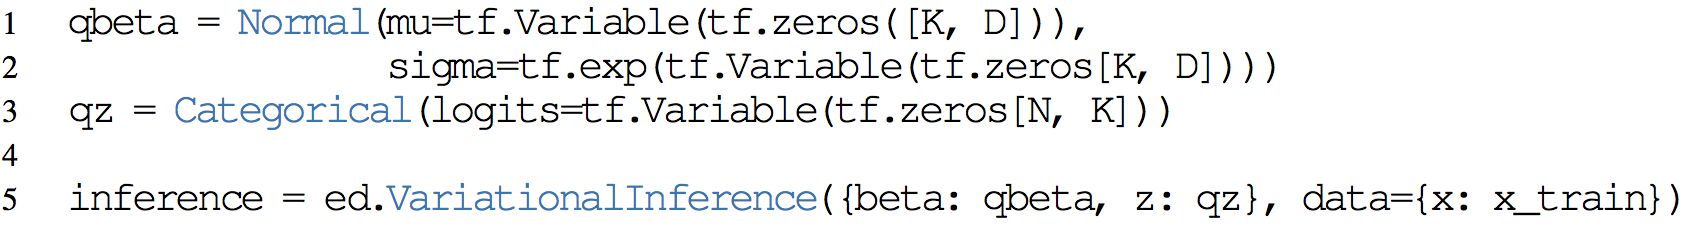
\includegraphics[height=5.25cm]{img/inference_variational.png}
\item
Specific variational algorithms inherit from
\texttt{VariationalInference} to define their own methods,
e.g., a
loss function and gradient.
\item
Monte Carlo approximates the posterior using samples.
We represent it where
the approximating family is an empirical distribution,
$q(\beta; \{\beta^{(t)}\}) = \frac{1}{T}\sum_{t=1}^T \delta(\beta,
\beta^{(t)})$,
$q(\mbz; \{\mbz^{(t)}\}) = \frac{1}{T}\sum_{t=1}^T \delta(\mbz,
\mbz^{(t)})$.

\vspace{1ex}
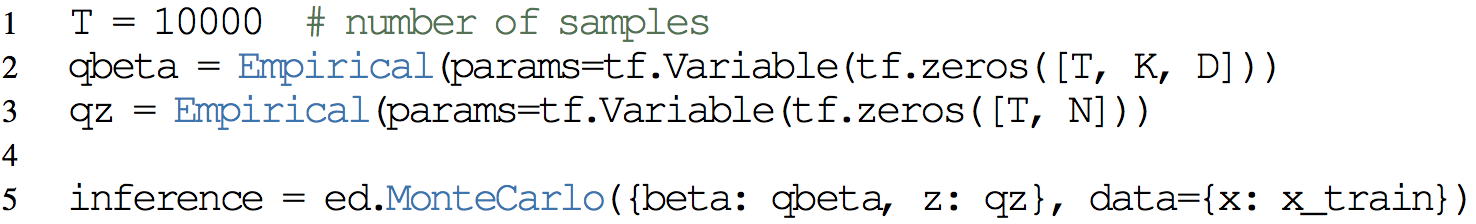
\includegraphics[height=5.25cm]{img/inference_monte.png}
\item
Monte Carlo
algorithms proceed by updating one sample $\beta^{(t)},\mbz^{(t)}$ at a time in the empirical
approximation.
Specific \glsunset{MC}\gls{MC} samplers determine the update rules.
\end{itemize}
\end{block}

\end{column}

\begin{column}{\sepwid}\end{column} % Empty spacer column

\begin{column}{\onecolwid}

\begin{block}{Example: Variational Auto-Encoder}
\begin{tabular}{cc}
\hspace{-2.15em}
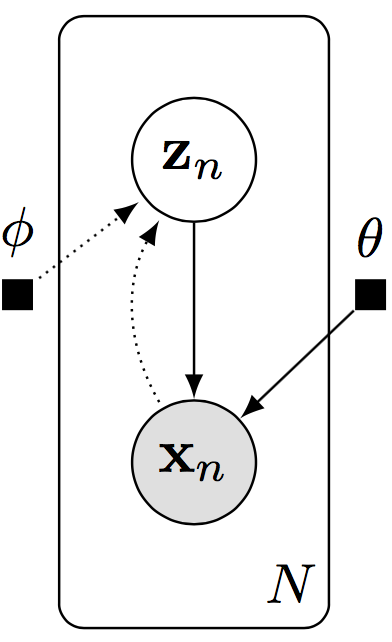
\includegraphics{img/vae_graph.png}
&
\hspace{-0.5em}
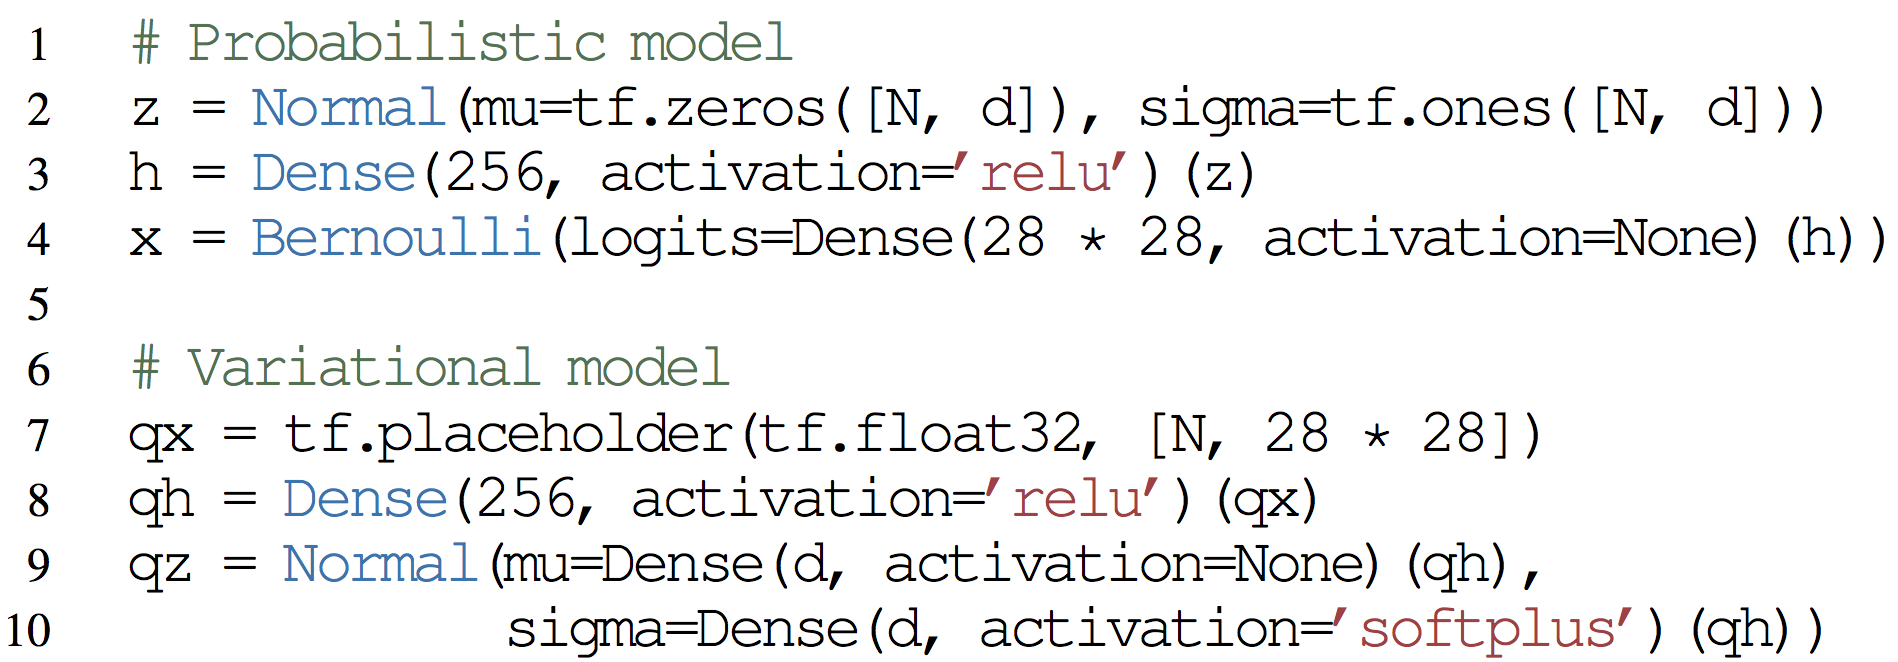
\includegraphics[width=0.85\textwidth]{img/vae_code.png}
\end{tabular}
\vspace{-2ex}
\end{block}

\begin{block}{Example: Generative Adversarial Networks}
\begin{tabular}{cc}
\hspace{-1.5em}
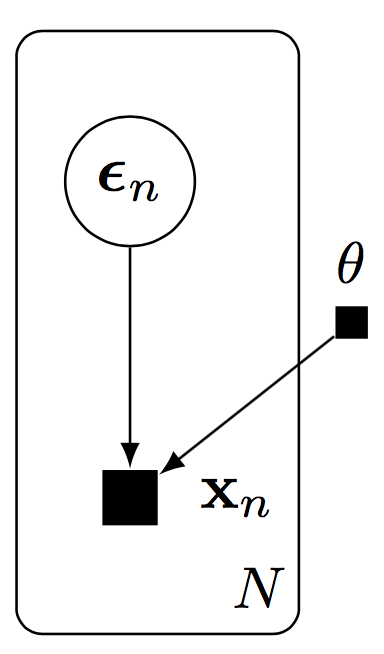
\includegraphics{img/gan_graph.png}
&
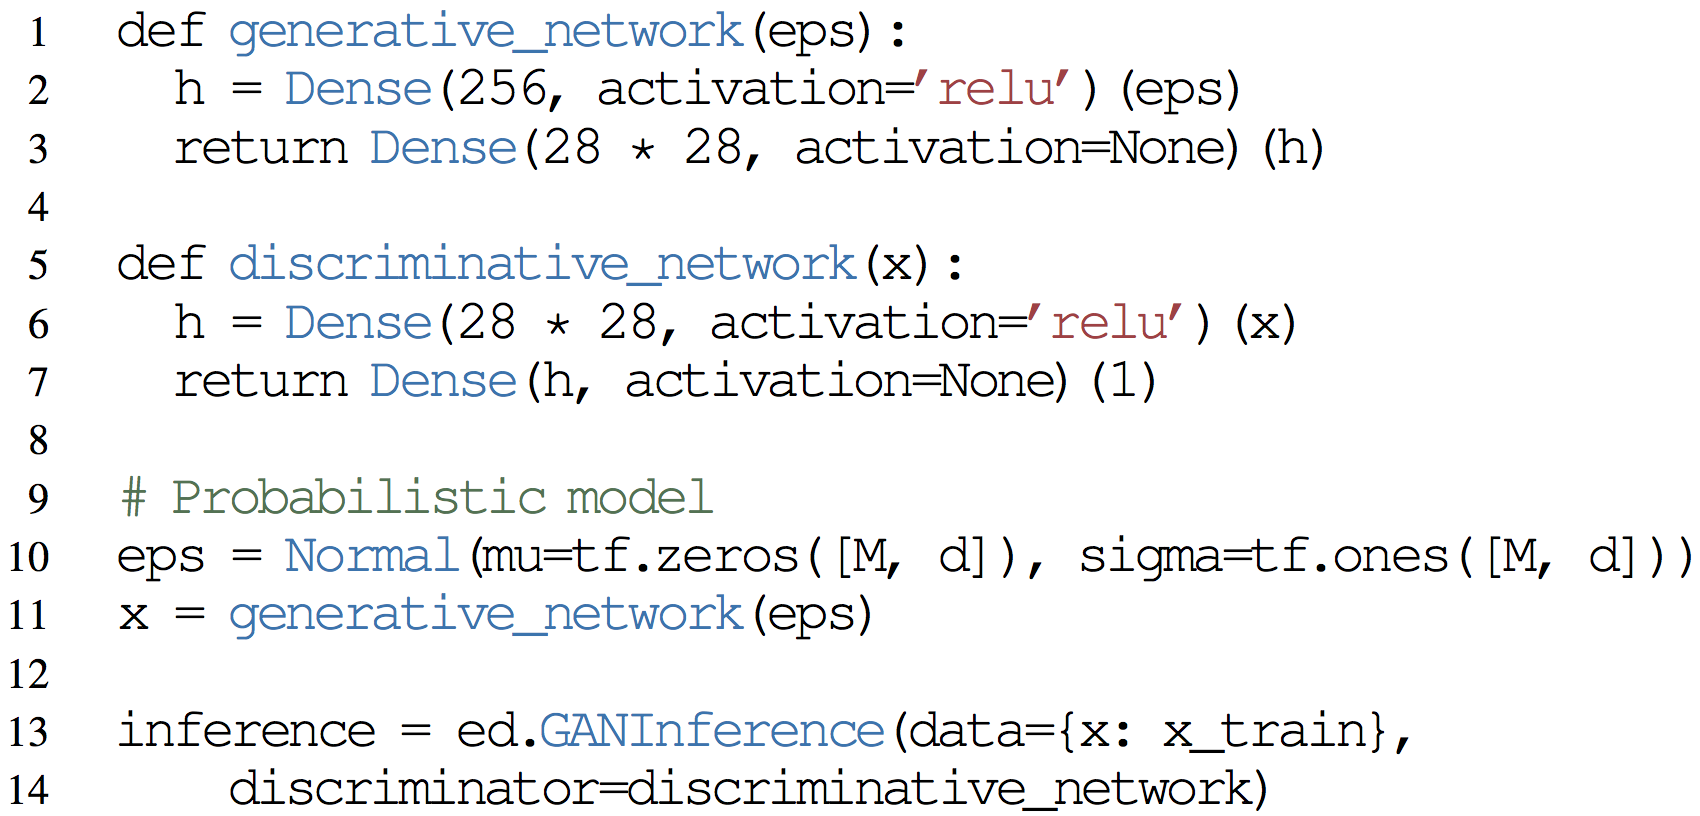
\includegraphics[width=0.77\textwidth]{img/gan_code.png}
\end{tabular}
\vspace{-2ex}
\end{block}

\begin{block}{Example: Bayesian RNN with Variable Length}
\begin{tabular}{cc}
\hspace{-1.5em}
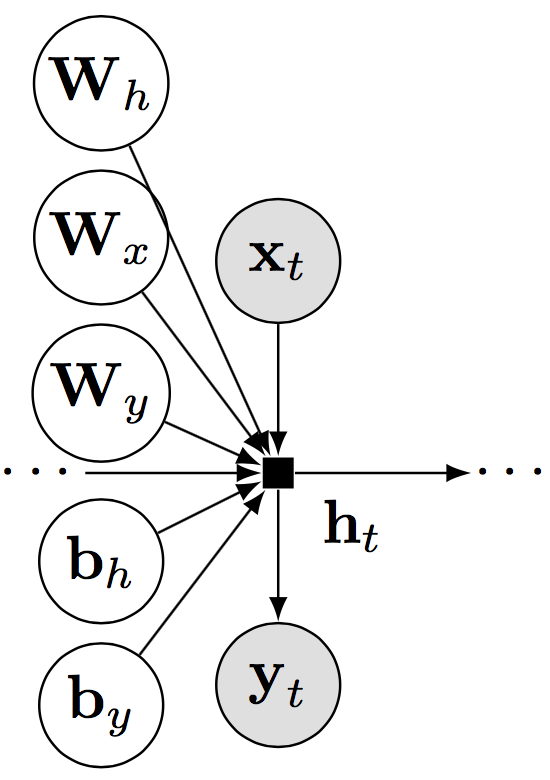
\includegraphics{img/bayesian_rnn_graph.png}
&
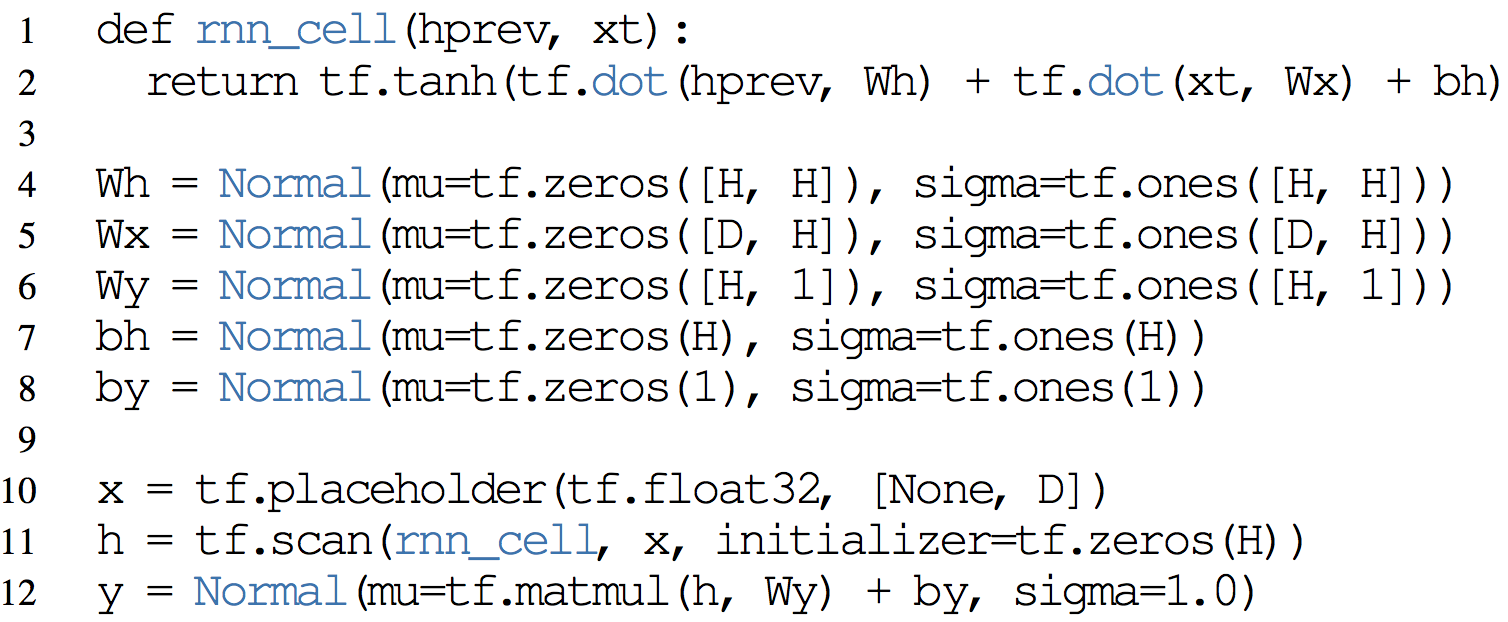
\includegraphics[width=0.80\textwidth]{img/bayesian_rnn_code.png}
\end{tabular}
\vspace{-2ex}
\end{block}

\begin{block}{Composing Inferences}
Core to Edward's design is that inference can be written as a collection
of separate inference programs. Below we demonstrate variational EM.
\vspace{1ex}

\begin{center}
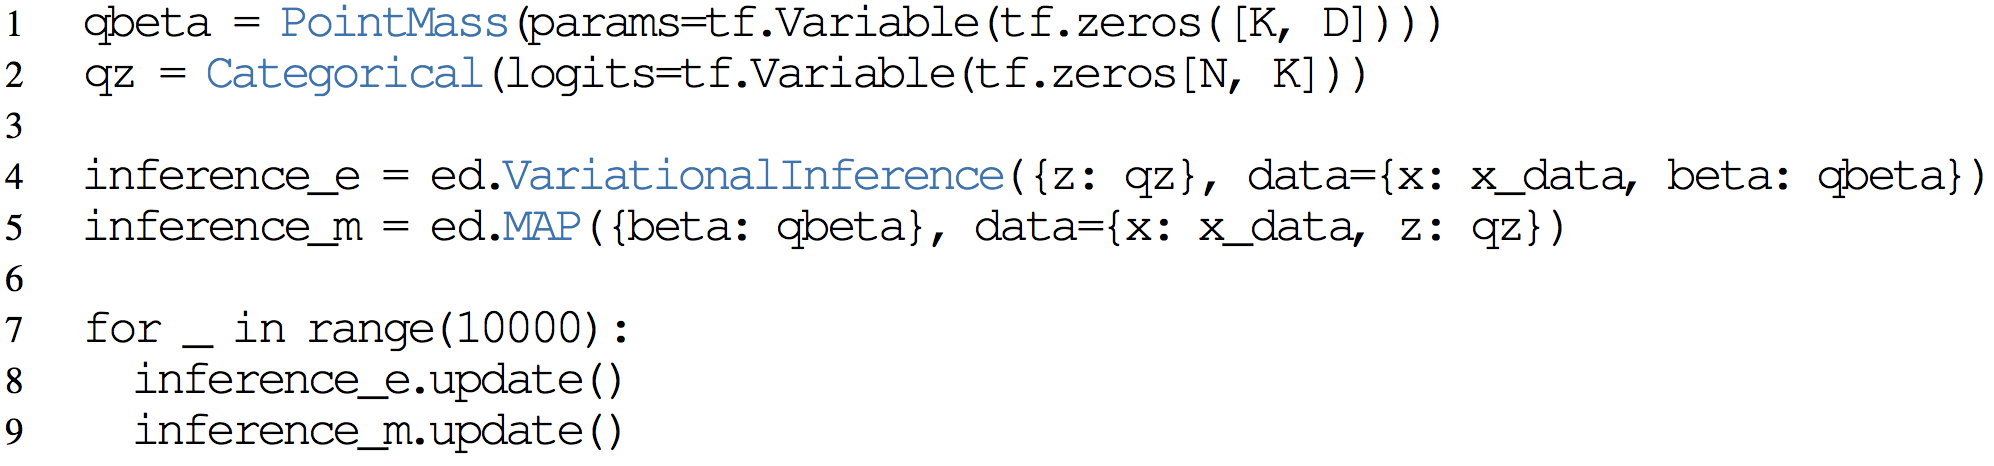
\includegraphics{img/composing.png}
\end{center}

\end{block}

\end{column}

\begin{column}{\sepwid}\end{column} % Empty spacer column

\begin{column}{\onecolwid}

\begin{block}{Experiments: Recent Methods in Variational Inference}
\begin{table}[tb]
\centering
\begin{tabular}{lcc}
\toprule
Inference method & Negative log-likelihood
\\
\midrule
\Gls{VAE} \citep{kingma2014autoencoding} & $\le$ 88.2 \\
\gls{VAE} without analytic KL & $\le$ 89.4 \\
\gls{VAE} with analytic entropy & $\le$ 88.1 \\
\gls{VAE} with score function gradient & $\le$ 87.9 \\
Normalizing flows \citep{rezende2015variational} & $\le$ 85.8 \\
Hierarchical variational model \citep{ranganath2016hierarchical} & $\le$ 85.4 \\
Importance-weighted auto-encoders ($K=50$) \citep{burda2016importance}
& $\le$ 86.3 \\
\acrshort{HVM} with \acrshort{IWAE} objective ($K=5$)
& $\le$ 85.2 \\
R\'{e}nyi divergence ($\alpha=-1$) % \citep{li2016variational}
& $\le$ 140.5 \\
%\gls{GAN} objective \citep{goodfellow2014generative}& -- \\
\bottomrule
\end{tabular}
\end{table}

Inference methods for a probabilistic decoder on binarized
MNIST. The Edward \acrshort{PPL} makes it easy to experiment with many algorithms.
\end{block}

\begin{block}{Experiments: GPU-accelerated Hamiltonian Monte Carlo}
\begin{tabular}{cc}
\hspace{-1em}
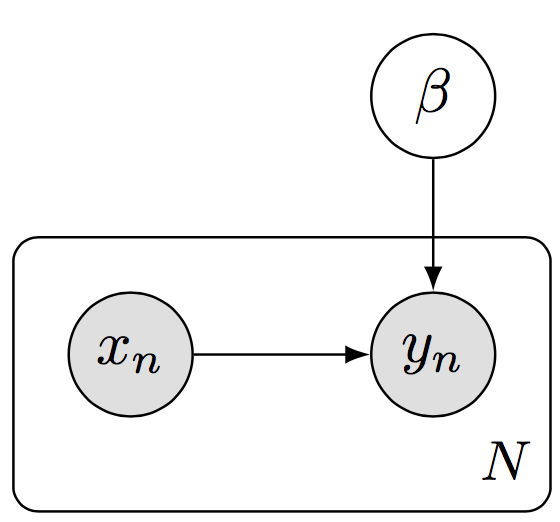
\includegraphics{img/logistic_graph.png}
&
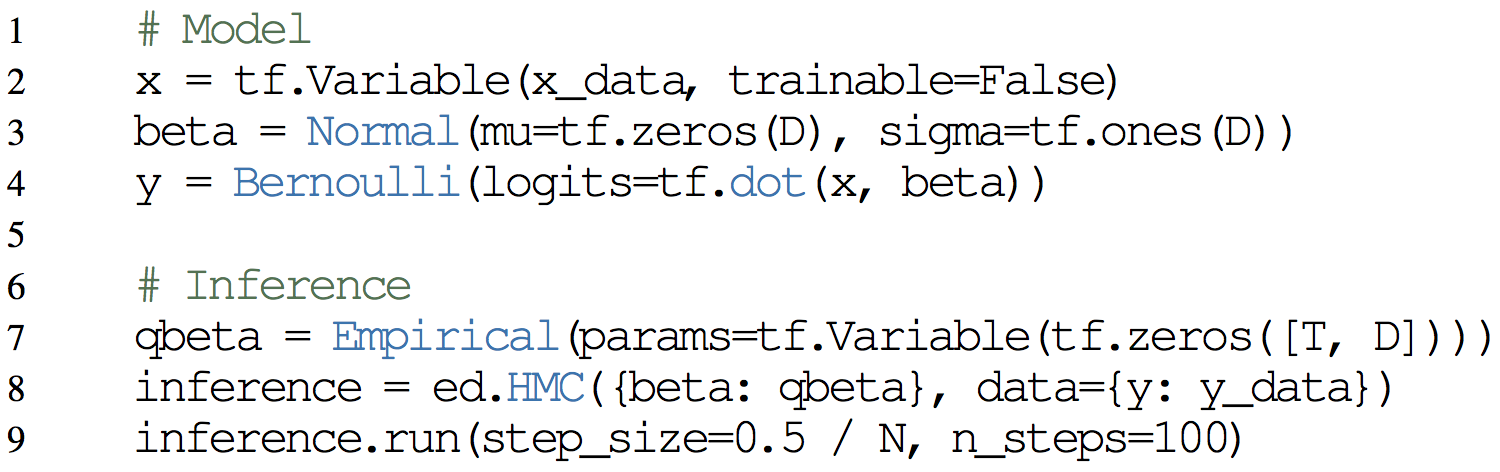
\includegraphics{img/logistic_code.png}
\end{tabular}
\vspace{1ex}

We perform inference on Bayesian logistic regression for the
Covertype dataset ($N=581012$, $D=54$). We use a 12-core Intel i7-5930K
CPU at 3.50GHz and a NVIDIA Titan X (Maxwell) GPU.

We compare the runtime of HMC for 100 iterations (and same settings).
\vspace{1ex}

\begin{table}[tb]
\centering
\begin{tabular}{ll}
\toprule
Probabilistic programming language & Runtime
\\
\midrule
Stan (1 CPU) \citep{carpenter2016stan} & 171 sec \\
PyMC3 (12 CPU) \citep{salvatier2015probabilistic} & 361 sec \\
\textbf{Edward (12 CPU)} & \textbf{8.2 sec} \\
\textbf{Edward (GPU)} & \textbf{4.9 sec} (35x faster than Stan)\\
\bottomrule
\end{tabular}
\end{table}
\end{block}

\vspace{-2ex}
\begin{block}{References}
\small{\bibliographystyle{apalike}
\bibliography{BIB}\vspace{0.75in}}
\end{block}

\end{column}

\begin{column}{\sepwid}\end{column} % Empty spacer column

\end{columns} % End of all the columns in the poster
\end{frame}   % End of the enclosing frame
\end{document}
